\chapter{Практическая часть}
\label{ch:chap2}

\section{Реализация градиентного спуска с постоянным шагом (learning rate)}
\label{sec:fig}

\textbf{Сейчас и в последующем будем считать, что $\varepsilon = 10^{-6}$, в крайних случаях, если значение изменится, об этом будет сказано}

\begin{lstlisting}[language=Python, caption=Функция градиента]
import numpy as np
import scipy
import matplotlib.pyplot as plt

eps = 1e-6

def grad(f,x):
    h = 1e-6
    l = f(x[:,np.newaxis] + h * np.eye(x.size))
    r = f(x[:,np.newaxis] - h * np.eye(x.size));
    return (l - r)/(2*h)
\end{lstlisting}

\begin{lstlisting}[language=Python, caption=Градиентный спуск]
def gradient_descent(f,x,lr,lim=2000):
    points = []
    points.append(x)
    while f(x) - f(x - lr * (g := grad(f,x))) > eps:
        x = x - lr * g
        points.append(x)
        if len(points) > lim:
          return np.array([])
    return np.array(points)
\end{lstlisting}

\begin{lstlisting}[language=Python]
def f(x):
    return (x[0] - 2) ** 2 + (x[1] + 3) ** 2
t = np.linspace(-10,10,100)
X, Y = np.meshgrid(t,t)
ax = plt.figure().add_subplot(projection='3d')
ax.set_xlabel("x")
ax.set_ylabel("y")
ax.set_zlabel("f(x,y)")
ax.plot_surface(X, Y, f(np.stack((X, Y))))
\end{lstlisting}

\newpage

\begin{figure}[ht]
    \centering
    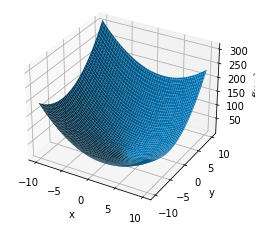
\includegraphics[width=0.5\textwidth]{images/gd1.png}
    \caption{Функция и ее график}
    \label{fig:gd1}
\end{figure}

\begin{lstlisting}[language=Python]
lr = 0.1
x = np.array([-1,1])
points = gradient_descent(f,x,lr)
print("x = ",points[-1])
print("f(x) = ",f(points[-1]))
plt.plot(points[:, 0], points[:, 1], 'o-')
plt.contour(X, Y, f([X, Y]), levels=sorted([f(p) for p in points]))
\end{lstlisting}

\begin{figure}[ht]
    \centering
    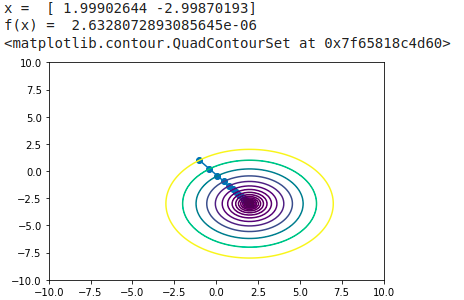
\includegraphics[width=0.5\textwidth]{images/gd2.png}
    \caption{Графическая интерпретация итераций алгоритма}
    \label{fig:gd2}
\end{figure}

\newpage

\section{Реализация градиентного спуска на основе одномерного поиска}

\subsection{Метод дихотомии}

\begin{lstlisting}[language=Python]
def f(x):
    return (x / 16 - 1) ** 2 * (2 * x ** 3 - 15 * x) - x ** 2

alpha = 12
beta = 19
t = np.linspace(alpha,beta,10000)
y = (0.2 * t - 1) * (0.2 * t - 6) ** 3 + 70
plt.plot(t,f(t))
plt.xlabel("x")
plt.ylabel("f(x)")
plt.show()
\end{lstlisting}

\begin{figure}[ht]
    \centering
    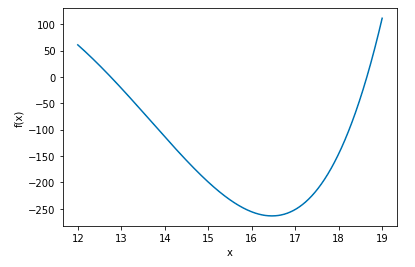
\includegraphics[width=0.5\textwidth]{images/t21.png}
    \caption{Берем произвольную функцию одного переменного}
    \label{fig:t21}
\end{figure}

\begin{lstlisting}[language=Python]
x = [alpha,beta]

points = []
points.append(x[::])

# Dichotomy algorithm
while (x[1] - x[0]) > eps:
    delta = eps / 2
    x1 = (x[0] + x[1]) / 2 - delta / 2
    x2 = (x[0] + x[1]) / 2 + delta / 2
    if f(x1) < f(x2):
        x[1] = x2
    else: 
        x[0] = x1
    points.append(x[::])

points = np.array(points)

ax1 = plt.subplot(1, 2, 1)
ax2 = plt.subplot(1, 2, 2)
ax1.set_xlabel("x")
ax2.set_xlabel("x")
ax1.set_ylabel("f(x)")
ax2.set_ylabel("f(x)")
pos1 = ax2.get_position()
ax2.set_position([pos1.x0 + 0.1,
                  pos1.y0,
                  pos1.width,
                  pos1.height])
ax1.scatter((points[::,0] + points[::,1]) / 2,f((points[::,0] + points[::,1]) / 2,), color='red')
ax1.plot(t,f(t))
ax2.plot(f((points[::,0] + points[::,1]) / 2))
\end{lstlisting}

\begin{figure}[ht]
    \centering
    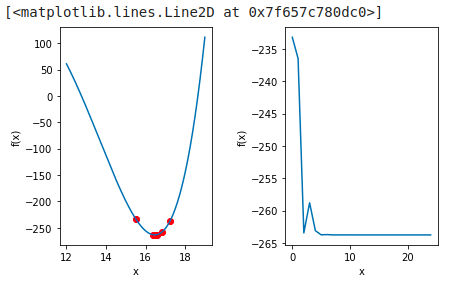
\includegraphics[width=0.5\textwidth]{images/t22.png}
    \caption{Пример работы дихотомии}
    \label{fig:t222}
\end{figure}

\newpage

\subsection{Модифицированный градиентный спуск}

\begin{lstlisting}[language=Python]
def dichotomy(f,a,b):
    x = np.array([a,b])
    while dist(x[0],x[1]) > eps:
        delta = (x[1] - x[0]) / 2
        x1 = (x[0] + x[1]) / 2 - delta / 2
        x2 = (x[0] + x[1]) / 2 + delta / 2
        new_x = np.copy(x)
        if f(x1) < f(x2):
            new_x[1] = x2
        else:
            new_x[0] = x1
        x = new_x

    return (x[0] + x[1]) / 2
    
def gradient_descent_with_dichotomy(f,x,lr,lim=2000):
    points = []
    points.append(x)
    while f(x) - f(x - lr * (g := grad(f,x))) > eps:
        x = dichotomy(f,x,x - lr * g)
        points.append(x)
        if len(points) > lim:
          return np.array([])
    return np.array(points)
\end{lstlisting}
\newpage
Функция №1

$f(x,y) = \frac{1}{50}x^2 + 50y^2$

\begin{figure}[ht]
    \centering
    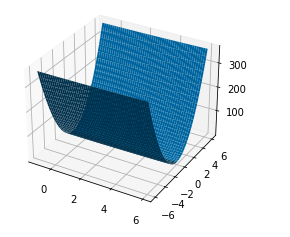
\includegraphics[width=0.5\textwidth]{images/g10.png}
    \caption{График функции}
    \label{fig:g10}
\end{figure}

\begin{figure}[ht]
    \centering
    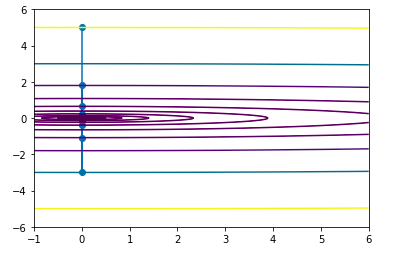
\includegraphics[width=0.5\textwidth]{images/g11.png}
    \caption{Работа ГС с постоянным шагом}
    \label{fig:g11}
\end{figure}

\begin{figure}[ht]
    \centering
    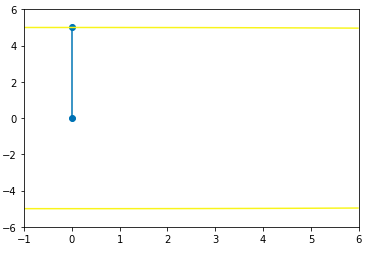
\includegraphics[width=0.5\textwidth]{images/g12.png}
    \caption{Работа ГС на основе дихотомии}
    \label{fig:g12}
\end{figure}

\newpage

Функция №2

$f(x,y) = \frac{1}{10}x^2 + 10y^2$

\begin{figure}[ht]
    \centering
    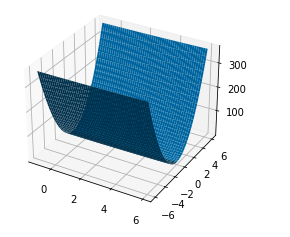
\includegraphics[width=0.5\textwidth]{images/g10.png}
    \caption{График функции}
    \label{fig:g10}
\end{figure}

\begin{figure}[ht]
    \centering
    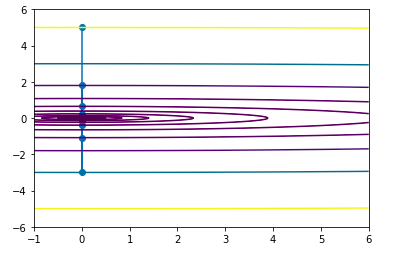
\includegraphics[width=0.5\textwidth]{images/g11.png}
    \caption{Работа ГС с постоянным шагом}
    \label{fig:g11}
\end{figure}

\begin{figure}[ht]
    \centering
    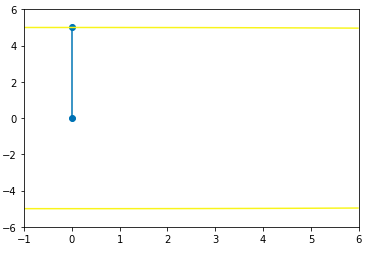
\includegraphics[width=0.5\textwidth]{images/g12.png}
    \caption{Работа ГС на основе дихотомии}
    \label{fig:g12}
\end{figure}

\newpage

Функция №3

$f(x,y) = (x^2 + y - 11)^2 + (x + y^2 - 7)^2$

\begin{figure}[ht]
    \centering
    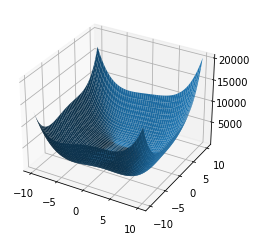
\includegraphics[width=0.5\textwidth]{images/g30.png}
    \caption{График функции}
    \label{fig:g30}
\end{figure}

\begin{figure}[ht]
    \centering
    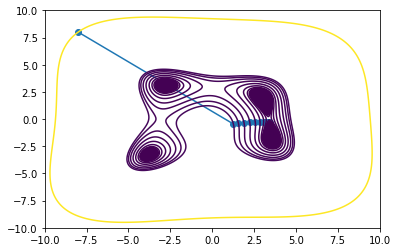
\includegraphics[width=0.5\textwidth]{images/g31.png}
    \caption{Работа ГС с постоянным шагом}
    \label{fig:g31}
\end{figure}

\newpage

\begin{figure}[ht]
    \centering
    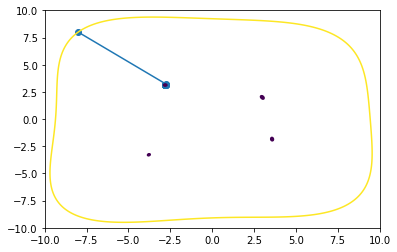
\includegraphics[width=0.5\textwidth]{images/g32.png}
    \caption{Работа ГС на основе дихотомии}
    \label{fig:g32}
\end{figure}

\begin{landscape}
\section{Дополнительные исследования}
\begin{vplace}[1.0]
\begin{figure}[ht]
    \centering
    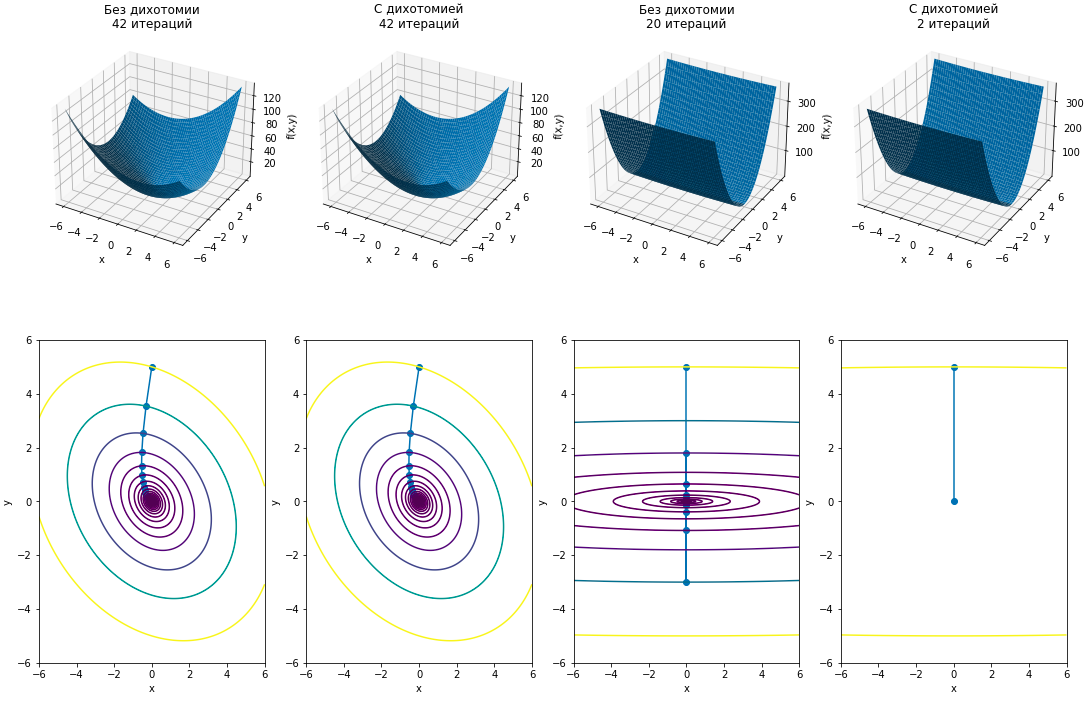
\includegraphics[width=1.0\textwidth]{images/4a.png}
    \caption{Сравнение количества итераций алгоритмов ГС}
    \label{fig:4a}
\end{figure}
\end{vplace}
\end{landscape}


Количество вызовов функции и подсчетов градиентов для данных случаев:
    \begin{enumerate}
    \item Вызовы функции: 132 \\
    Подсчеты градиента: 33
    \item Вызовы функции: 2230 \\
    Подсчеты градиента: 33
    \item Вызовы функции: 80 \\
    Подсчеты градиента: 20
    \item Вызовы функции: 120 \\
    Подсчеты градиента: 2
    \end{enumerate}
\begin{landscape}
\begin{vplace}[1.0]
\begin{figure}[ht]
    \centering
    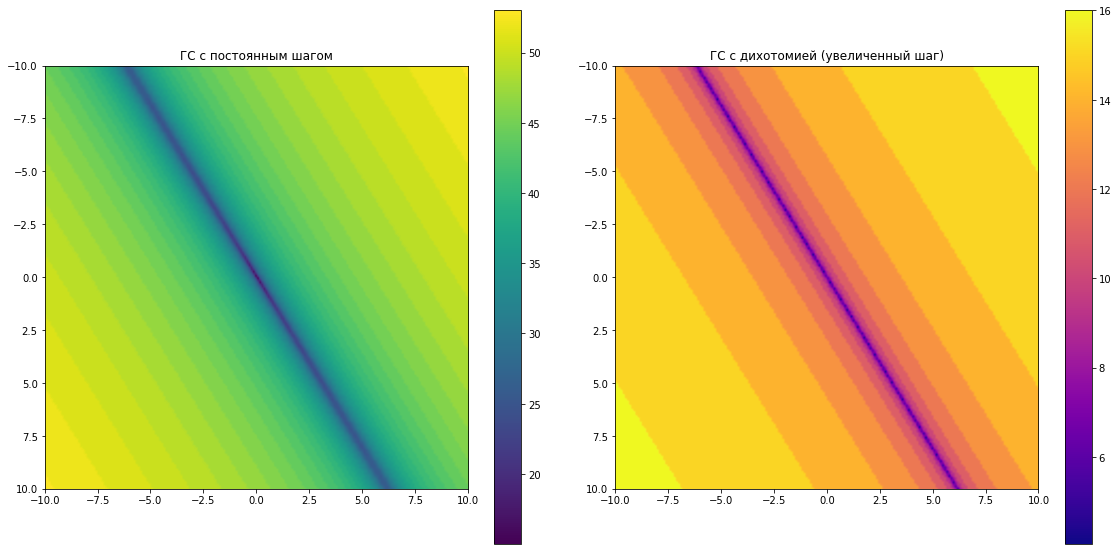
\includegraphics[width=1.5\textwidth]{images/4c.png}
    \caption{Количество итераций алгоритмов ГС в зависимости от выбора начальной точки}
    \label{fig:4c}
\end{figure}
\end{vplace}
\end{landscape}
\begin{landscape}
\begin{vplace}[1.0]
\begin{figure}[ht]
    \centering
    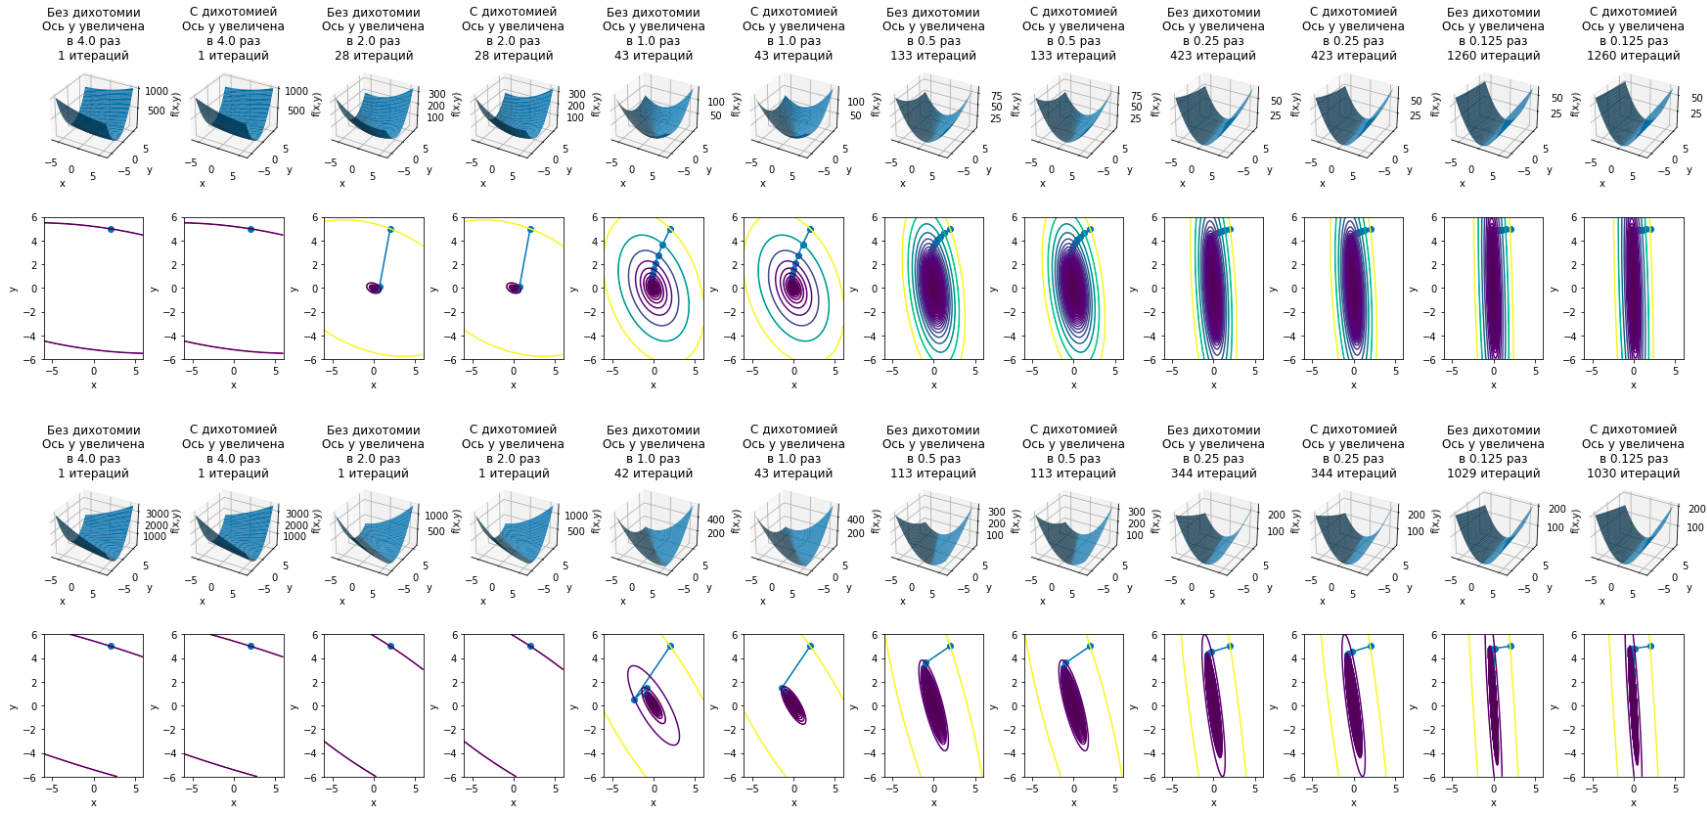
\includegraphics[width=1.5\textwidth]{images/4d.png}
    \caption{Количество итераций алгоритмов ГС в зависимости от масштабирования осей}
    \label{fig:4d}
\end{figure}
\end{vplace}
\end{landscape}
\section{Анализ градиентного спуска и его модификации на основе дихотомии}

Эффективность градиентного спуска сильно зависит от выбора шага. Если шаг будет слишком большой, то алгоритм градиентного спуска может "перескочить" точку минимума (См. графики функций 1 и 2), что приведет к лишним итерациям алгоритма, а в крайне плохих плохих случаях к тому, что градиентный спуск не будет сходиться.

Модификация градиентного спуска с использованием дихотомии позволяет алгоритму сходиться в таких случаях, причем значительно быстрее, чем сходится градиентный спуск с постоянным шагом. Однако если шаг слишком мал, то результат модифицированного алгоритма не будет отличаться от обычного градиентного спуска ничем, кроме времени исполнения, которое у модифицированного алгоритма будет значительно больше (см. дополнительное исследование 1).

На примере функции №3 мы можем заметить, что обычный и модифицированый градиентный спуск могут вернуть различные точки минимума. (В данном случае это не является проблемой, так как приведенная функция имеет 4 точки минимума с равными значениями функции в них.)

Если шаг слишком маленький, то это так же может приводить к лишним итерациям алгоритма. В дополнительном исследовании 2 в каждом тесте не изменялись никакие переменные, кроме точки запуска алгоритма, которая отдалялась от точки минимума, что приводило к увеличению времени исполнения алгоритмов. 

Ускорить выполнение можно с помощью нормализации осей функции. По результатам дополнительного исследования можно увидеть, что существуют случаи, когда методы ГС не сходятся или сходятся за очень большое количество итераций, и это можно исправить с помощью нормализации.

\section{Реализация генератора квадратичных функций $n$ переменных с числом обусловленности $k$}

\begin{lstlisting}[language=Python]
# Quadratic function generation
def gen_f(n,k):
    m = np.random.rand(n, n) * 2
    Q, _ = np.linalg.qr(m)
    D = np.diag(np.array([k] + [1] * (n - 1)))

    result = Q @ D @ np.linalg.inv(Q)
    def f_impl(x):
        return x.T @ result @ x

    def f(x):
        return np.apply_along_axis(f_impl, 0, x)
        
    return f

def gen_f_poly(n,k):
    m = np.random.rand(n, n) * 2
    Q, _ = np.linalg.qr(m)
    D = np.diag(np.array([k] + [1] * (n - 1)))

    result = Q @ D @ np.linalg.inv(Q)
    
    parts = []
    for i in range(n):
      for j in range(n):
        x = f'x{i}^2' if i == j else f'x{i}*x{j}'
        parts.append(f'{result[i][j]}*{x}')

    return ' + '.join(parts)

gen_f_poly(2, 1000)
\end{lstlisting}

\begin{figure}[ht]
    \centering
    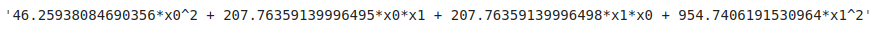
\includegraphics[width=0.5\textwidth]{images/gen1.png}
    \caption{Генератор функций, вывод сгенерированной функции в виде полинома}
    \label{fig:gen1}
\end{figure}

\begin{figure}[ht]
    \centering
    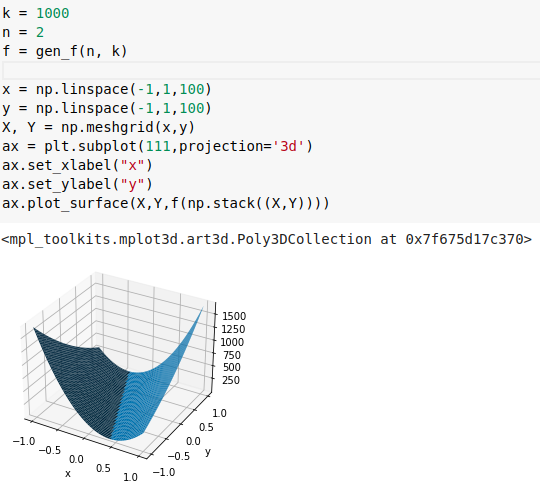
\includegraphics[width=0.5\textwidth]{images/gen2.png}
    \caption{Пример работы генерации функции для $n=2$ и $k=1000$}
    \label{fig:gen2}
\end{figure}

\section{Исследование зависимости числа итераций, необходимых градиетному спуску для сходимости}

\begin{figure}[ht]
    \centering
    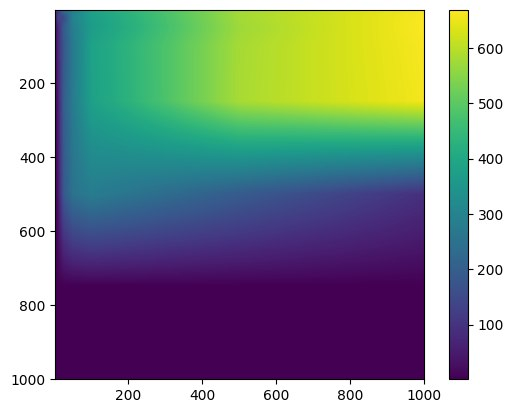
\includegraphics[width=0.5\textwidth]{images/task6-7.jpg}
    \caption{Тепловая карта значений $T(n,k)$ (по горизонтали - n, по вертикали - k)}
    \label{fig:task6-7}
\end{figure}

\section{Реализация одномерного поиска с условием Вольфе}

\begin{lstlisting}[language=Python, caption=Проверка условия Вольфе]
def check_wolfe(f, x, alpha, dir, c1=0.1, c2=0.9):
  gx = grad(f, x)
  cond1 = f(x + alpha*dir) <= f(x) + alpha * c1 * np.dot(dir, gx)
  cond2 = abs(np.dot(dir, grad(f, x + alpha * dir))) <= abs(c2 * np.dot(dir, gx))
  return cond1 and cond2
\end{lstlisting}


\begin{lstlisting}[language=Python, caption=Нахождение коэффициента для условия Вольфе и градиентный спуск на основе условия Вольфе]
def find_wolfe(f, x, dir):
    m = mk = 1
    start_alpha = 0.5
    for m in range(1, 20):
        alpha = start_alpha ** m
        if check_wolfe(f, x, alpha, dir):
          mk = m
          break
    return start_alpha ** mk

def gradient_descent_wolfe(f,x,lim=2000):
    points = []
    points.append(x)
    g = grad(f, x)
    if (np.linalg.norm(g) < 1e-6):
      return np.array(points)
    alpha = find_wolfe(f, x, -g)
    while f(x) - f(x - alpha * g) > 1e-6:
        x = x - alpha * g
        points.append(x)
        if len(points) > lim:
          return np.array([])
        g = grad(f, x)
        if (np.linalg.norm(g) < 1e-6):
          return np.array(points)
        alpha = find_wolfe(f, x, -g)
    return np.array(points)
\end{lstlisting}



\begin{landscape}
\begin{vplace}[1.0]    
\begin{figure}[ht]
    \centering
    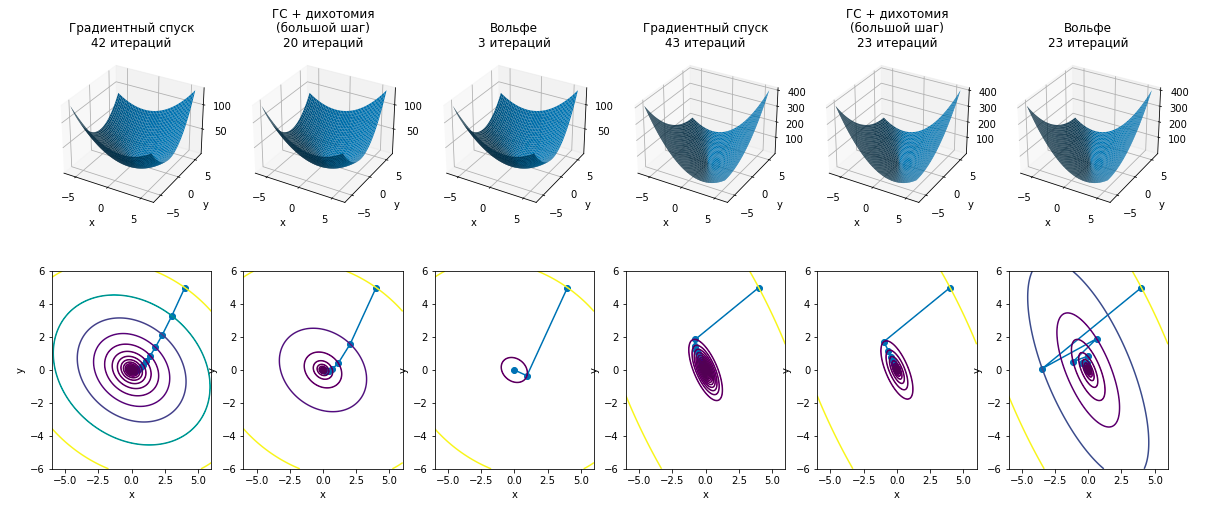
\includegraphics[width=1.5\textwidth]{images/w4.png}
    \caption{Сравнение методов}
    \label{fig:w4}
\end{figure}
\end{vplace}
\end{landscape}

\endinput